\section{Enunciare la legge di Amp\'ere ed usarla per il calcolo
	del campo magnetico all'interno di un solenoide rettilineo
	percorso da corrente stazionaria.}
Secondo la \textbf{Legge di Amp\'ere}:
$$
    \Gamma_B = \mu_0 I_{conc}
$$
Dove :
\begin{itemize}
	\item [$\Gamma_B$] {
		\`e la circuitazione del campo magnetico $B$ sulla    linea chiusa $l$, ovvero :
        $$
            \Gamma_B = \oint_l{\vec{B}} = \oint{\vec{B} \cdot d\vec{l}}
        $$
    }
    \item [$I_{conc}$] {
    	\`e la somma delle correnti concatenate al percorso \textbf{chiuso} su cui si esegue la circuitazione.
    }
\end{itemize}
\begin{center}
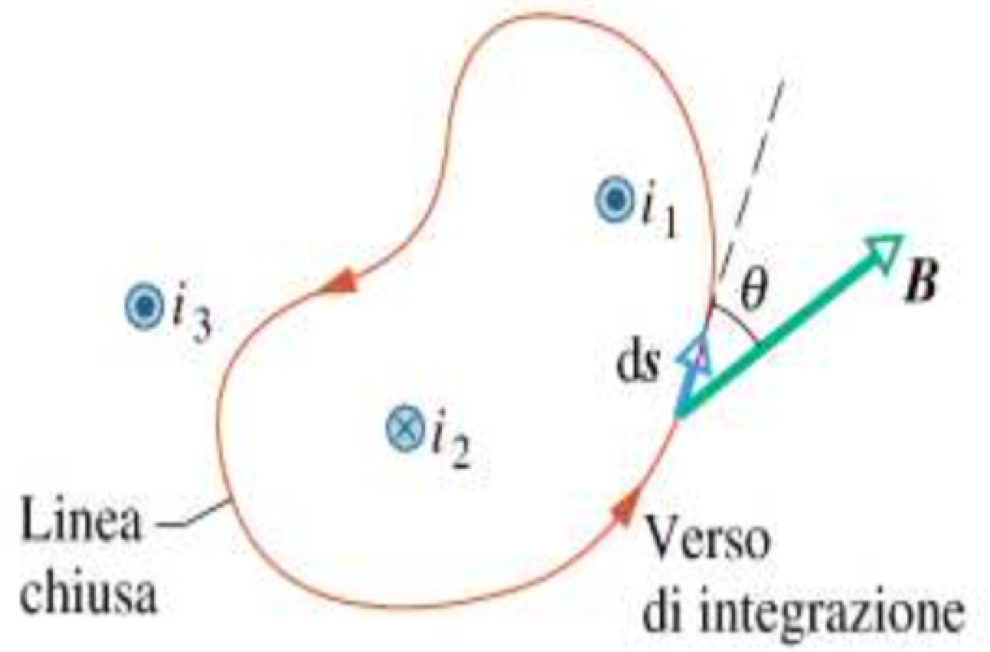
\includegraphics[width=0.6\textwidth]{ampere_1}
\end{center}

\pagebreak

Un esempio di applicazione consiste nel considerare un solenoide lungo $l$ avente $n$ spire per unit\'a di lunghezza. \\
Esso \`e percorso da un campo magnetico $\vec{B}$ uniforme, dove le sue linee sono orientate parallelamente all'asse. Scegliamo la circuitazione come un quadrato di lato $h$ lungo i punti $a$, $b$, $c$, $d$ come da immagine.
\begin{center}
	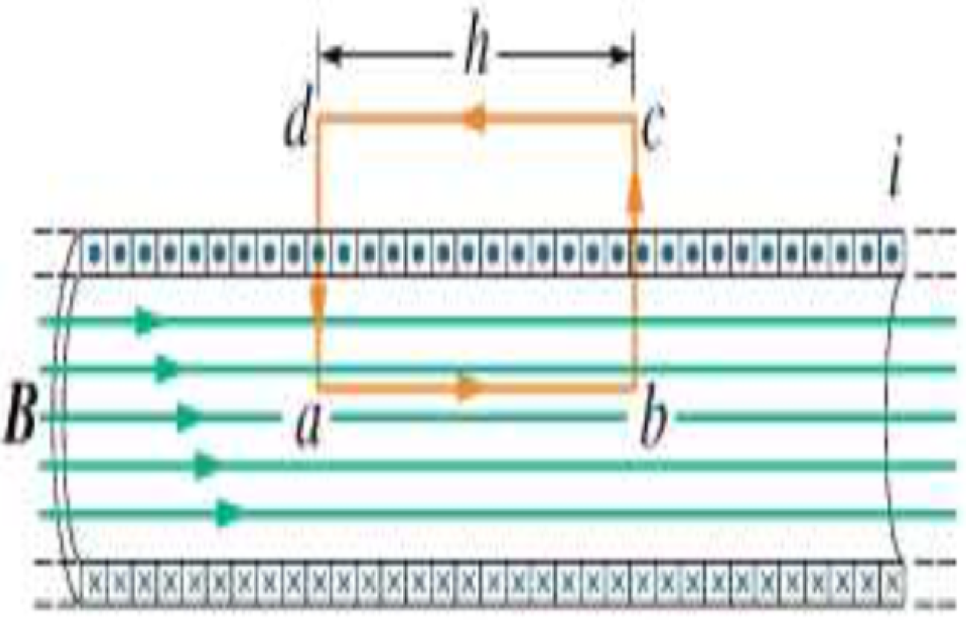
\includegraphics[width=0.6\textwidth]{ampere_2}
\end{center}
Abbiamo quindi che:
$$
     \Gamma_B = \oint_{abcd}{\vec{B}} = \oint_{ab}{\vec{B}} + \oint_{bc}{\vec{B}} + \oint_{cd}{\vec{B}} + \oint_{da}{\vec{B}}
$$
Da cui assumiamo che : 
\begin{itemize}
	\item [$\oint_{cd}{\vec{B}} = 0$] {
	    Poich\'e $cd$ non \`e all'interno del solenoide.	
	}
	\item [$\oint_{bc}{\vec{B}} = \oint_{da}{\vec{B}} = 0$] {
		Poich\'e $\vec{bc} \perp \vec{B} \land da \perp \vec{B} \land \vec{V_1} \perp \vec{V_2} \Longrightarrow \vec{V_1} \cdot \vec{V_2} = 0$
	}
	\item [$\oint_{ab}{\vec{B}}$] {
		Siccome $\vec{ab} \parallel \vec{B}$ vale che:
		$$
	        \oint_{ab}{\vec{B}} = \int{\vec{B} \cdot d\vec{ab}} = Bh
		$$
	}
\end{itemize}
Sfruttando questo eguagliamo:
$$
    \Gamma_B = \oint_{abcd}{\vec{B}} = \oint_{ab}{\vec{B}} = Bh
$$
$$
    Bh = \mu_0 I_{conc}
$$
Da cui si conclude che :
$$
    B = \mu_0 \frac{I_{conc}}{h} = \mu_0 \frac{n \cancel{h} i}{\cancel{h}} = \mu_0 n i
$$
Dove : 
\begin{itemize}
	\item [n] {\`e il numero di spire per unit\'a di lunghezza }
	\item [i] {\`e la corrente che scorre nel solenoide}
\end{itemize}
Si noti che : $I_{conc} = n h i$.
$\hfill\square$